% !TeX spellcheck = en_US
\section{Deep Learning for SISR and noise reduction}\label{sec:deep_learning}

\subsection{Deep Learning for Single Image Super-Resolution}
Recently, deep learning methods for \gls{sisr} have demonstrated promising performance and accuracy compared to conventional \gls{sisr} algorithms. Before \gls{srcnn} \cite{SRCNN} was presented, which is the pioneer work in the field, Yang et al. \cite{SISRBENCH} categorized \gls{sisr} algorithms in 4 groups based on the image prior:
\begin{itemize}
	\item Prediction models, that apply a predefined mathematical formula to generate \gls{hr} outputs without training data. Bilinear, bicubic and Lanczos interpolation methods are examples of algorithms in this group.
	\item Edge based methods, that learn priors from edge features in order to predict \gls{hr} images from \gls{lr} images.
	\item Image statistical methods, that use statistical properties of the images as priors to reconstruct the \gls{hr} images.
	\item Patch based methods, that learn mapping functions from sets of paired \gls{lr} and \gls{hr} training images.
\end{itemize}

With the publication of \gls{srcnn} \cite{SRCNN}, deep learning methods can be added to this taxonomy. Within this category, multiple methods using different kinds of neural network have been developed. 

Kim et al. proposed \gls{vdsr} \cite{VDSR}, that uses a similar structure as \gls{srcnn} but using a deeper network.

\gls{espcn} \cite{ESPCN} was proposed by Shi et al. to make \gls{srcnn} more efficient. This network performs the feature extraction in the \gls{lr} space in order to consume less computational resources. Once the extraction is done, it uses a sub-pixel convolution in order to reconstruct the \gls{hr} image.

Dong et al. designed \gls{fsrcnn} \cite{FSRCNN} by accelerating \gls{srcnn} \cite{SRCNN} in multiple steps. First, the last convolution layer of \gls{srcnn} was replaced by a deconvolution layer, eliminating the need for using bicubic interpolation on the input \gls{lr} image. Second, the non-linear mapping layer was replaced by a shrinking layer, 4 non-linear mapping layers and an expanding layer, increasing the number of layers but reducing the number of parameters.

Residual networks have also been used for the \gls{sisr} task \cite{EDSR}\cite{REDNET}. These networks use skip connections to jump over some of their layers in order to tackle the problem of gradient vanishing, allowing to design very deep networks.

Lai et al. proposed \gls{lapsrn} \cite{LAPSRN}\cite{LAPSRN2}, based on a Laplacian pyramid framework, that progressively reconstructs the sub-band residuals from its feature extraction branch in order to obtain the \gls{hr} images. 

Some image denoisers, such as \gls{ircnn} \cite{IRCNN} and \gls{dncnn} \cite{DNCNN} also address the problem of \gls{sisr}. These methods model the image degradation in the \gls{sisr} problem by taking the noise as the difference between the \gls{hr} image and the bicubic upsampling of the \gls{lr} image.
 
\gls{gan} have also been used for \gls{sisr} \cite{SRGAN}. In these models, two neural networks contest with each other, in the context of game theory, in order to solve the super-resolution problem. The generative network generates output data by super-resolving \gls{lr} images and the discriminative network evaluates them. The objective of the discriminative network is to distinguish between real \gls{hr} images and super-resolved images while the generative network tries to increase its error rate.

Anwar et al. \cite{DBLP:SISR} proposed a taxonomy that categorizes deep learning methods for \gls{sisr} into 9 different groups according to their model designs, namely, linear networks, residual networks, recursive networks, progressive reconstruction designs, densely connected networks, multi-branch designs, attention based networks, multiple degradation handling networks and \gls{gan} models.

\subsection{Deep Learning for Image Denoising}
Image denoising is another important task in computer vision applications. Over the past years, multiple methods for modeling image priors, such as \gls{mrf} \cite{MRF}, \gls{bm3d} \cite{BM3D} and \gls{ncsr} \cite{NCSR}, have been proposed in order to tackle this problem. However, the mentioned methods have shown high computational cost and they also need to have their parameters manually chosen in order to improve the performance \cite{DBLP:DEEPNR}. Multiple methods have been proposed to solve these problems. 

In \cite{TNRD}, Chen et al. presented a  \gls{tnrd} model in which the filters and the influence functions can be learned from the training data. 

In \cite{DEEPAM}, Kim et al. proposed \gls{deepam}, which learns a regularizer via deep aggregation in order to solve multiple image restoration tasks, including single image denoising.  

Zhang et al. proposed \gls{dncnn} \cite{DNCNN}, which uses residual learning and batch normalization in order to speed up the training process and boost the denoising performance.

Zhang et al. also proposed \gls{ircnn} \cite{IRCNN}, which is a \gls{cnn}-based image denoiser that can be used for several low-level computer vision tasks such as \gls{sisr} or deblurring. \gls{ircnn} uses \gls{hqs} to show that a \gls{cnn} based denoiser prior can be plugged as a modular part of model-based optimization methods in order to solve multiple inverse problems.

In \cite{DILATED}, Wang et al. present a dilated residual \gls{cnn} for Gaussian image denoising in which the receptive field is enlarged by adopting dilated convolution.

\subsection{FSRCNN and IRCNN}
In this subsection, we review the structure of the two \glspl{cnn} used in this study: \gls{fsrcnn} and \gls{ircnn}.

\subsubsection{FSRCNN} The structure of \gls{fsrcnn} is composed of 5 different parts. The first four are made up of convolution layers and the last one is a deconvolution layer:

\begin{figure}
	\centering
	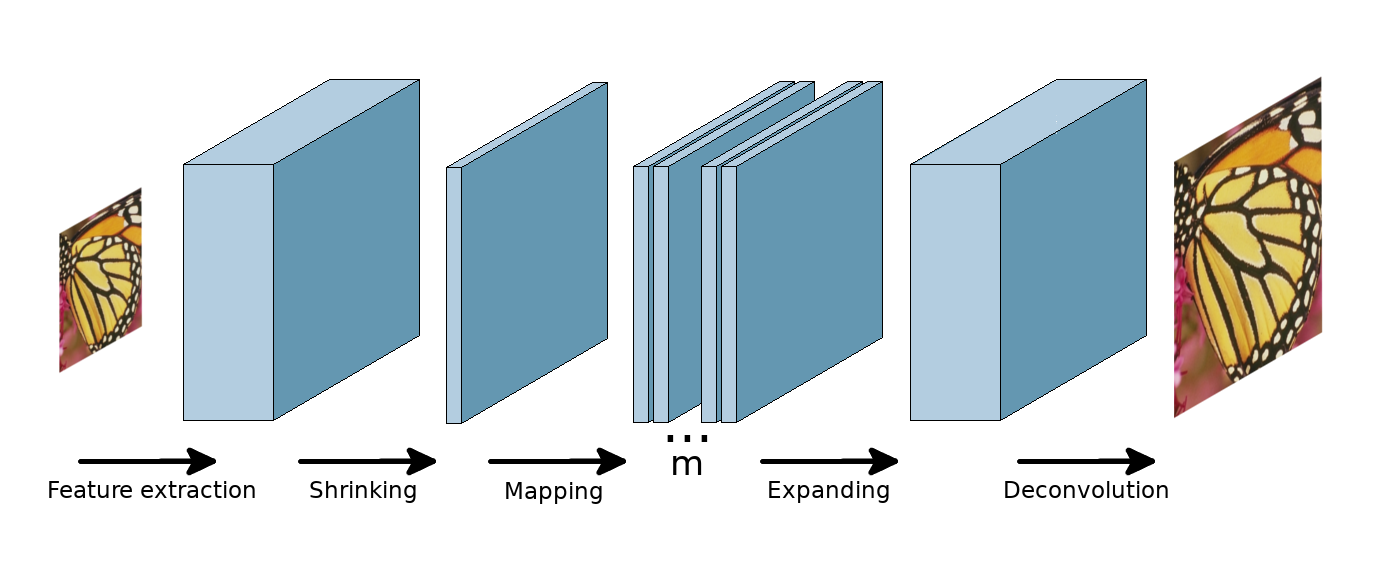
\includegraphics[width=0.7\textwidth]{images/fsrcnn.png}
	\caption{Structure of \gls{fsrcnn}}
	\label{fig:fsrcnn}
\end{figure}

\begin{itemize}
	\item \textbf{Feature extraction}. This operation extracts overlapping patches from the \gls{lr} input by convolving them with a set of $d$ filters that represent each patch as a high dimensional feature vector. The size of the filters proposed by the authors for this layer is $5$. On the other hand, the input number of channels is $1$.
	
	\item \textbf{Shrinking}. A shrinking layer is added after the feature extraction in order to reduce the \gls{lr} feature dimension by convolving the \gls{lr} features with $s$ filters of size $1$. With this filter size, linear combinations applied in the  \gls{lr} feature space reduce its dimension from $d$ to $s$, decreasing as well the number of parameters and therefore the computational cost.
	
	\item \textbf{Non-linear mapping}. This operation maps each high-dimensional feature vector onto another high-dimensional feature vector by applying $m$ convolution layers with $s$ filters of size $3$. The resulting vectors represent the \gls{hr} version of the extracted patches.
	
	\item \textbf{Expanding}. A expanding layer is added after the non-linear mapping process in order to expand the \gls{hr} feature dimension that was previously reduced by the shrinking layer. Since this operation acts as the inverse process of the shrinking step, $d$ filters of size $1$ are applied in order to perform the expansion.
	
	\item \textbf{Deconvolution}. The last step in the process consists of applying a deconvolution layer in order to perform the upsampling operation and the aggregation of the features. This layer applies $1$ deconvolution filter of size $9$ using the upscale factor as the deconvolution stride in order to directly produce the \gls{hr} image as an output.
\end{itemize}

The described architecture is shown in Figure \ref{fig:fsrcnn}.

Following the notation proposed in \cite{FSRCNN}, we denote the convolution layers as $Conv(f_i, n_i, c_i)$ and the deconvolution layer as $DeConv(f_i, n_i, c_i)$ where $f_i$ is the size of the filter, $n_i$ is the number of filters and $c_i$ is the number of channels in the $i-th$ layer. Using this notation, we can describe the structure as:

\begin{flalign}
\nonumber\text{LR image} \rightarrow & \underbrace{Conv(5,d,1) + PReLU}_{\text{Feature extraction}} \rightarrow \underbrace{Conv(1, s, d) + PReLU}_{\text{Shrinking}} \\\nonumber
\rightarrow & \underbrace{m\times\left(Conv(3,s,s) + PReLU\right)}_{\text{Non-linear mapping}} \rightarrow \underbrace{Conv(1,d,s) + PReLU}_{\text{Expanding}} \\\nonumber
\rightarrow & DeConv(9,1,d) \rightarrow \text{HR image}
\end{flalign}

where \gls{prelu} \cite{PRELU} is the activation function used. With this structure, there are three variables that need to be chosen and they will directly affect the performance of the network: the mapping depth $m$, the \gls{lr} feature dimension $d$ and the number of shrinking filters $s$.

\subsubsection{IRCNN} The structure of \gls{ircnn} consists of seven different convolutional layers divided in three parts.

\begin{figure}[h]
	\centering
	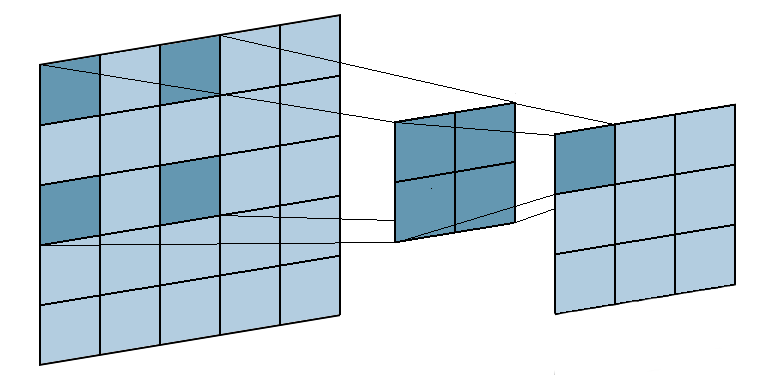
\includegraphics[width=0.5\textwidth]{images/dilated.png}
	\caption{Dilated convolution of a $5\times5$ matrix with a $2\times2$ kernel using a dilation factor of 2. The operation results in a $3\times3$ matrix.}
	\label{fig:dilated}
\end{figure}

\begin{itemize}
	\item The first layer is a convolution layer with 64 filters of size $3$ that uses \gls{relu} as the activation function.
	\item The following 5 layers are dilated convolution layers with 64 filters of size $3$ that use batch normalization \cite{BATCHNORM} in order to accelerate the training and improve its stability. \gls{relu} is also used as the activation function of these layers. 
	
	The dilated convolution layers apply dilated convolution operations in order to capture the context information. The dilation factors of the dilated convolution layers are 2, 3, 4, 3 and 2 respectively. Figure \ref{fig:dilated} shows an example of a dilated convolution with a dilation factor of 2.
	
	\item The last layer is a convolution layer with $c$ filters of size $3$, where $c$ is the output depth.
\end{itemize}

\begin{figure}[h]
	\centering
	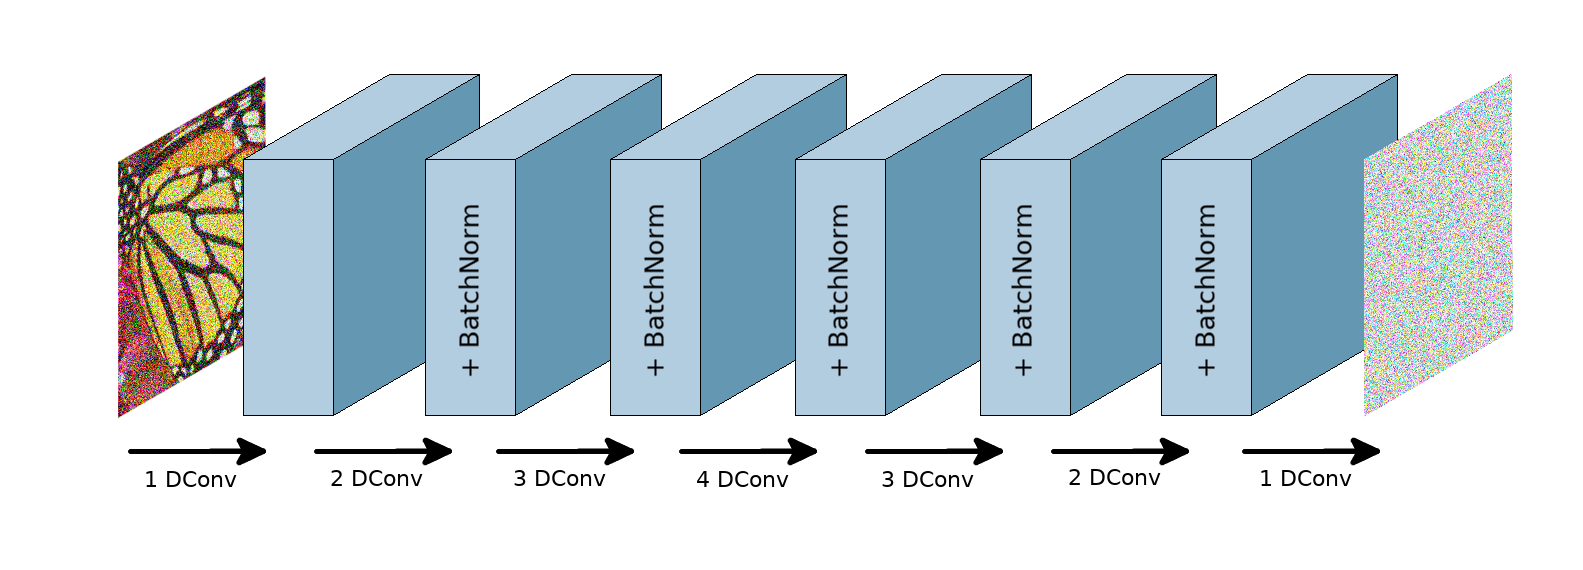
\includegraphics[width=0.7\textwidth]{images/ircnn.png}
	\caption{Structure of \gls{ircnn}}
	\label{fig:ircnn}
\end{figure}

The described architecture is shown in Figure \ref{fig:ircnn}. In the figure, the output of the network is the residual image, that represents the noise to be removed.

Following the notation described above, we represent a the dilated convolution layers as $DConv_{d_i}(f_i, n_i, c_i)$  where $d$ is the dilation factor, $f_i$ is the size of the filter, $n_i$ is the number of filters and $c_i$ is the number of channels in the $i-th$ layer.

\begin{flalign}
	\nonumber\text{LR image} \rightarrow & DConv_1(3,64,c)\\\nonumber
		\rightarrow & DConv_2(3,64,64) + BatchNorm + ReLU
		\rightarrow DConv_3(3,64,64) + BatchNorm + ReLU\\\nonumber
		\rightarrow & DConv_4(3,64,64) + BatchNorm + ReLU
		\rightarrow DConv_3(3,64,64) + BatchNorm + ReLU\\\nonumber
		\rightarrow & DConv_2(3,64,64) + BatchNorm + ReLU
		\rightarrow DConv_1(3,c,64) \rightarrow \text{Residual Image}
\end{flalign}